\documentclass[ngerman,runningheads,a4paper]{llncs}
\usepackage{graphicx}
\begin{document}

\title{Supporting Drum Learning/Playing through the use of Haptic Wearables}
\author{Simon Pfeifer}
\institute{Karlsruher Institut für Technologie, Institut für Telematik, Pervasive Computing Systems / TECO, Karlsruhe, Germany}
\maketitle

\begin{abstract}
Das Erlernen eines Musikinstruments ist eine lange und traditionell mühsame Aufgabe.
Haptische Wearables sollen den Lernprozess schneller und interessanter gestalten.
Das Schlagzeugspielen kann, durch die Verwendung aller vier Gliedmaßen, gut genutzt werden, um den Einsatz von haptischen Wearables zu testen.
Dabei kann aktiv gelernt werden, oder passiv während man sich mit einer anderen Aufgabe auseinandersetzt.
Grundlegende Entwurfsideen sind dafür das Haptic Drum Kit, sowie der Haptic iPod.
In dieser Arbeit gebe ich einen Überblick über die aktuell existierenden Technologien und Entwicklungsmöglichkeiten.
\end{abstract}

\begin{keywords}
drum learning, rhythm skills, haptic learning, multi-limb coordination, passive learning
\end{keywords}

\section{Einleitung}
Das Erlernen eines Musikinstruments ist eine lange und traditionell mühsame Aufgabe, besonders am Anfang, wenn die Ausgabe nicht sehr angenehm für die Ohren ist. Wearables bieten verschiedene Arten der Unterstützung, um den Lernprozess zu fördern, z.B. durch passives haptisches Lernen. Das Erlernen eines rhythmischen Instruments wie z.B. Schlagzeug könnte besonders geeignet sein, da eines der Haupthindernisse für Anfänger darin besteht, alle vier Gliedmaßen gleichzeitig und unabhängig voneinander in klar definierten, aufeinander bezogenen Mustern zu bewegen.
Das Erlernen eines Instruments ist schon immer ein langwieriger Prozess und hat sich im Laufe der Zeit nicht großartig gebessert.
Jeder hat sich schonmal ein bisschen an einem Instrument ausprobiert und versucht die ein oder anderen Töne, Tonfolgen oder ganze Lieder zustande zu bringen.
Das ganze frei nach Gehör oder mit entsprechender Ausbildung dann mit Noten.
Um einen Lehrer kommt man um effizient zu lernen fast nicht herum und durch die recht langsamen Fortschritte verlieren viele wieder die Lust und widmen sich lieber etwas anderem.
\newline
Die aktuelle Forschung versucht dem entgegenzuwirken durch neue Lernmethoden.
Unter anderem mit haptischen Wearables.
Hier werden haptischen Sensoren am Körper befestigt und durch einen Computer gesteuert.
Durch nachspielen des haptischen Feedbacks, soll einfacher und schneller Lernerfolg erreicht werden und somit auch die Motivation.
\newline
In dieser Arbeit möchte ich die Ergebnisse zusammenführen und einen Überblick über die aktuellen Forschungsergebnisse geben.
Ist es möglich durch haptische Wearables das Schlagzeugspielen zu lernen?
Lernt man auf diese Weise einfacher und schneller als durch auditives Lernen oder einen Lehrer?
Kann sich eine Musikgruppe durch ein haptisches Metronom im Tempo halten und muss nicht dauernd auf den Dirigenten oder die anderen Musiker achten?
Diese Fragen werden durch die Arbeit beantwortet und bilden den roten Faden.


\section{Grundlagen}

\subsection{Haptische Wahrnehmung}

\subsubsection{tactile Sense}

\subsubsection{force feedback}

\subsection{Haptische Sensoren}
Welche haptischen Sensoren gibt es
Wie funktionieren diese

\subsection{Haptic Wearables}
In welchen Wearables werden haptische Sensoren verbaut
Welche Funktionen werden dadurch verwirklicht bzw. ermöglicht

\section{Aktives Lernen mit Haptischen Wearables}

\subsection{Haptic Drum Kit}
In diesem Abschnitt geht es um das Haptic Drum Kit von Simon Holland, Anders J. Bouwer, Mathew Dalgleish und Topi M. Hurtig \cite{10.1145/1709886.1709892}
.
Diese Arbeit beschäftigt sich damit, ob sich polyphone Rhythmen, für die man mehrere Gliedmaßen koordinieren muss, durch Vibratoren an den Handgelenken und Knöcheln lernen lassen.
Unter polyphonen Rhythmen versteht man Rhythmen, die sich aus mehreren einfachen Rhythmen zusammensetzen, welche unterschiedlich schnell sein können.
Die Wissenschaftler untersuchen die Frage, ob Anfänger schwere Rhythmen nur mit haptischen Stimuli lernen können.
Zudem vergleichen sie, wie die Benutzer nur mit Audio, oder mit Audio und Haptik lernen.

\subsubsection{Aufbau}
Das Haptic Drum Kit besteht aus 4 Vibratoren, die mit elastischen Bändern an den Handgelenken und Knöcheln befestigt werden.
Die Sensoren werden an den Gliedmaßen angebracht, weil kein Transfer mehr nötig sein soll, um den richtigen Arm, oder das richtige Bein zu bewegen.
Mit einem Computer werden die Vibratoren angesteuert und der Benutzer soll diesen haptischen Signalen nachspielen.
Als Schlagzeug wird ein Midi drum kit verwendet, um die zeitliche Genauigkeit des Benutzers am Computer messen zu können.

\subsubsection{Ergebnisse}
Die Befragung der Probanden zeigte, dass alle gewillt waren, das System wieder zu benutzen und die Kombination von Audio und Haptik am besten fanden.
Entgegen dem gehofften Ergebnis waren die Benutzer mit Audio Anleitung besser im Takt und konnten einfacher mitmachen.
Es wurden auch viele Verbesserungvorschläge gebracht.
Die Vibratoren waren zu laut und die Vibration teilweise zu schwach und wurde so von der Bewegung des Schlages übertönt.
Die Sensoren sollten sich individuell einstellen lassen.
Bei schnellen Rhythmen können mehrere Vibrationen zu einer verschwimmen.
Durch die Gleiche Vibrationsintensität war auch schwer festzustellen, wo der Rhythmus beginnt, oder zur Wiederholung ansetzt.
Es wurde viel parallel gelernt, statt jede Bewegung alleine.
Eine neue Version des Haptic Drum Kits mit verbesserten Sensoren, die deutlicher, individuell und zeitlich präziser funktionieren, kann schon viele Probleme der ersten Version beheben.

\begin{figure}
  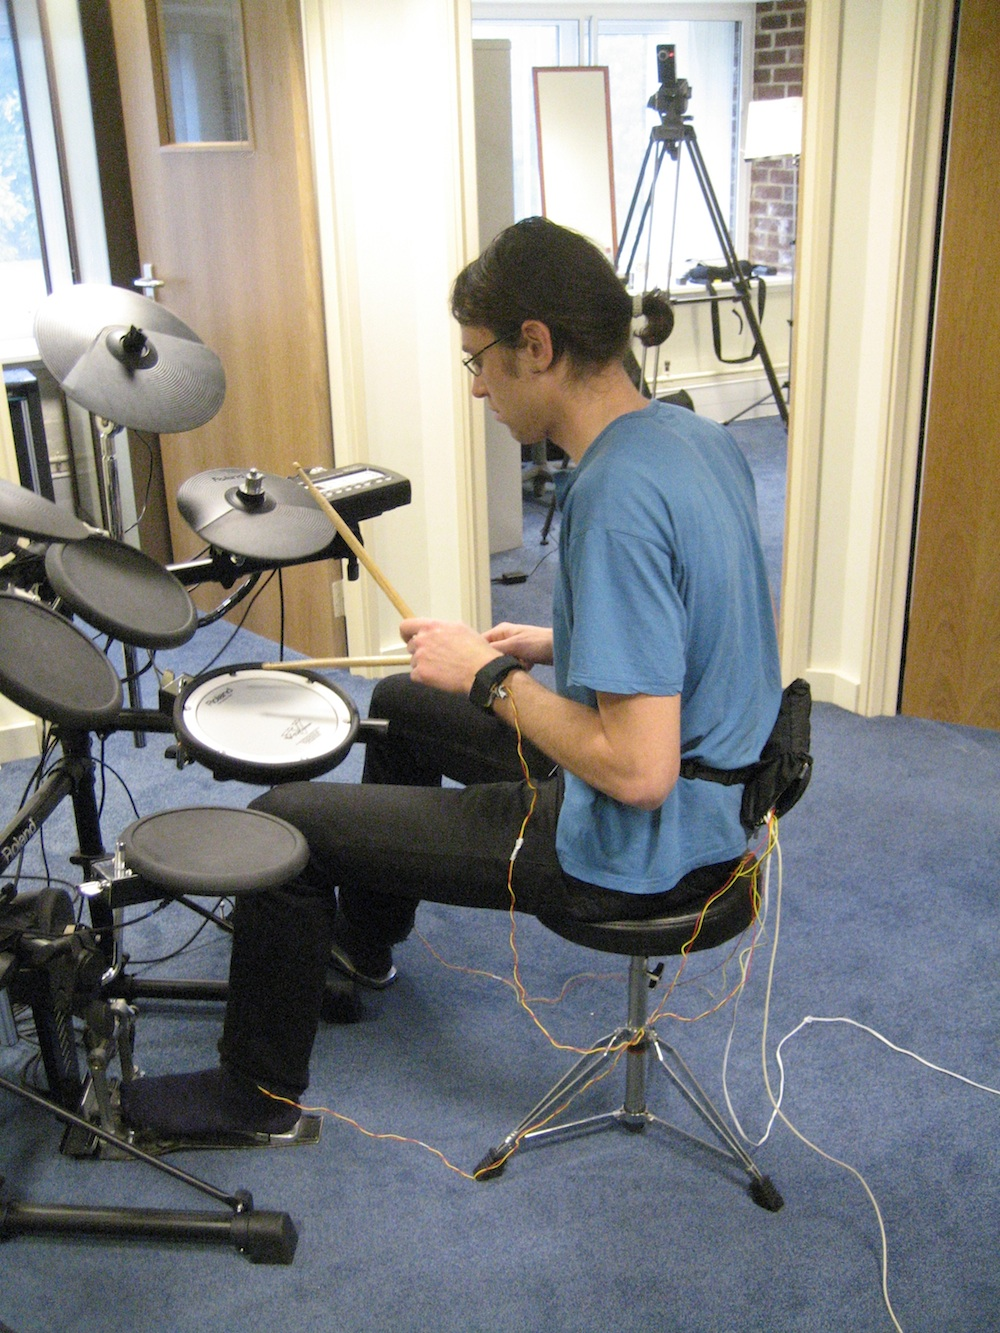
\includegraphics[width = \textwidth]{pictures/hapticdrumkit}
  \caption{Haptic Drum Kit \cite{10.1145/1709886.1709892}}
\end{figure}

\subsection{Haptic Drumstick}
Graham Grindlay \cite{4479984} zeigt in seiner Arbeit wie gut ein einfacher Rhythmus sich mit haptischer Führung lernen lässt.


\section{Passives Lernen durch Haptische Wearables}

\subsection{Haptic iPod}
Die Arbeit von Bouwer, Dalgleish und Holland\cite{bouwer2011haptic} basiert auf den Ergebnissen zum Haptic Drum Kit \cite{10.1145/1709886.1709892} und beschäftigt sich mit der Frage, ob sich mehrgliedrige Rhythmen auch passiv lernen lassen.
Dabei werden lautlos rhythmische Reize über die Haptischen Sensoren abgespielt, während sich die Probanden mit anderen Aufgaben beschäftigen.
Das verwendete System wird Haptic iPod genannt.
\subsubsection{Aufbau}
Der Haptic iPod existiert in zwei verschiedenen Versionen.
Eine portable Feldversion mit im Vorhinein aufgenommenen vierspurigen Stücken und batteriebetriebenen Kopfhörerverstärkern.
Dazu noch eine statische Testversion die mit einem Laptop bedient wird und mit stärkeren Kopfhörerverstärkern ausgestattet ist.
Für die Studie wurde die statische Testversion verwendet.
Die Probanden spielten zu Anfang möglichst schwere Rhythmen nach Gehör.
Danach wurden 2 Rhythmen aus den gespielten Rhythmen ausgewählt und abwechselnd über die haptischen Wearables abgespielt, während eine 30 minütige Leseverständnis Aufgabe bearbeitet wurde.
Im Anschluss sollten die Rhythmen vom Anfang wiederholt werden.
Die Ergebnisse wurden auf Genauigkeit, Timing, Anzahl der Versuche und Fehleranzahl im besten Versuch verglichen.
Zum Schluss wurden die Probanden zu ihren Erfahrungen und Einstellungen zum Haptic iPod befragt.

\subsubsection{Ergebnisse}
Wie auch beim Haptic Drum Kit \cite{10.1145/1709886.1709892} ist die Haptik gegenüber dem Gehör im Vorteil, wenn es darum geht, welche Gliedmaßen zu verwenden ist.
Es wurde sich auch die Kombination aus Gehör und Haptik gewünscht, wie auch Portabilität und Kabellosigkeit.
Die Haptik hat keinen Vorteil, wenn es darum geht, welche Trommel zu spielen ist und die Wearables sind über die Zeit unangenehm zu tragen gewesen.
Das passive Lernen macht es auch schwerer sich auf eine Aufgabe zu konzentrieren und fordert das setzen von Prioritäten.




Zwei Versionen: portable Feldversion und Statische Testversion
4 tactor vibrotactile devices secured to limbs
statische Version: laptop mit Behring Kopfhörer Verstärkern
portable Version: vorher aufgenommene 4 track audio mit batteriebetriebenen kopfhörer Verstärkern
stärkere statische version für tests verwendete
1 pre test möglichst schwere rhythmen nach audio als referenz
2 passive learning 2 rhythmen während leseverständnis 30 minuten
3 spielen der rhythmen von phase 1 mit den passiv gelernten rhythmen Vergleich anhand von genauigkeit, timing, Anzahl Versuche und Fehleranzahl in bestem versucht
4 Fragebogen mit Erfahrungen und Einstellungen zu haptischer Technologien
audio und haptik gleich welche trommel zu spielen Ist
haptik im vorteil, welche Gliedmaße zu benutzen Ist
haptik und audio als kombination gewünscht
geteilte Aufmerksamkeit fordert setzen von Priorität, schwerer zu konzentrieren
wearables über zeit unangenehm
rhythmus vor dem spielen durchdenken -> reduziert das lernen von falschen patterns



\section{Zusammenfassung}
\subsection{Ergebnisse}
\subsection{Ausblick}
weitere Anwendung von Haptik in Gesundheit, Unterhaltung, Sicherheit und weiteren Gebieten, die noch nicht identifiziert und untersucht wurden.
Erweiterung von smartphone Vibratoren, die fast nur an und aus kennen, könnte noch mehr Informationen übertragen.
Wireless haptic wearables weil die Kabel in der Bewegung einschränken und ein unangenehmes gefühl geben

\bibliographystyle{splncs03}
\bibliography{proseminar}
\end{document}
